% Course project report: Adaptive QUIC ACK-Frequency and Pacing Optimizer.
% Same template as the project proposal (proposal/Proposal1.pdf).
% Build: make (or: pdflatex report && pdflatex report)
\documentclass[11pt]{article}

\usepackage[letterpaper,margin=1in]{geometry}
\usepackage[T1]{fontenc}
\usepackage{times}
\usepackage{amsmath}
\usepackage{graphicx}
\usepackage{booktabs}
\usepackage{float}
\usepackage{flafter}   % a float never appears before the text that places it
\usepackage{placeins}  % \FloatBarrier keeps floats inside their (sub)section
\usepackage{tabularx}
\usepackage[font=small,labelfont=bf]{caption}
\usepackage{tikz}
\usetikzlibrary{arrows.meta}
\usepackage{url}
\usepackage{fancyhdr}
\usepackage{hyperref}

\hypersetup{
  pdftitle={Adaptive QUIC ACK-Frequency and Pacing Optimizer},
  pdfauthor={Kunal Umaji, Kaveenraj G, Aravindh Sriram Kumar A G},
  pdfsubject={Modern Networks course project report},
}
\graphicspath{{figures/}}
\setlength{\emergencystretch}{3em}

% Running header and footer as in the proposal (the title page keeps the plain style).
\setlength{\headheight}{14pt}
\pagestyle{fancy}
\fancyhf{}
\lhead{QUIC ACK-Frequency \& Pacing Optimizer}
\rhead{Modern Networks Course Project Report}
\cfoot{Page \thepage}

\newcommand{\pol}[1]{\texttt{#1}}            % policy, modifier or code identifier
\newcommand{\para}[1]{\textbf{#1}} % run-in paragraph heading (followed by a normal space)
\newcommand{\ms}{\,ms}
\newcommand{\mbps}{\,Mb/s}

\begin{document}

\title{\textbf{Adaptive QUIC ACK-Frequency and Pacing Optimizer}\\ {\large Course Project Report}}
\author{Kunal Umaji (CS25S020)\\ Kaveenraj G (CS25S029)\\ Aravindh Sriram Kumar A G (CS26S020)}
\date{November 2026\\[0.4em] {\normalsize Code and data: \url{https://github.com/kunalumaji/mcn26}}}
\maketitle

\begin{abstract}
QUIC encrypts and processes every ACK in user space, so ACKs cost CPU at both endpoints. The IETF
ACK Frequency extension lets a data sender request fewer ACKs but leaves open how few: fewer ACKs
save CPU, yet they delay the feedback that congestion control and loss detection depend on. We
implement in MsQuic a CPU-aware policy, \pol{adaptive}, that raises the ACK threshold $T$ only
under measured CPU pressure, plus modifiers that bound $T$ by the congestion window and scale the
ACK delay with the RTT. Over 460--660\mbps{} Wi-Fi, \pol{adaptive} keeps $T{=}2$ on an idle
server. Under moderate CPU load it cuts ACKs by 56\% and client ACK-generation time by 44\% without
lowering goodput or video QoE. On a CPU-starved server, large thresholds cause throughput
collapses, while the window and delay bounds keep baseline performance with about 40\% fewer ACKs.
On an emulated 100\mbps{} path under CPU load, \pol{adaptive} cuts server ACK-processing time by
60--65\% at no cost in goodput. With 0.1\% random loss, however, its CPU-driven threshold loses two thirds of the goodput.
Bounding $T$ by the congestion window and the RTT keeps 79--96\% of the baseline goodput at any
ceiling while still removing two thirds of the ACKs. Network state must therefore bound any
CPU-driven threshold.
\end{abstract}

\section{Introduction}
QUIC implements its transport in user space and encrypts every packet, including packets that
carry only ACKs. TCP ACKs are handled by the kernel with offload support. A QUIC ACK costs a system
call and encryption at the receiver, and decryption and parsing at the sender. Zhang et al.\
identify user-space receiver processing, and ACKs in particular, as a main reason why QUIC is
slower than TCP+TLS on fast links~\cite{zhang2024quic}. LiteQUIC measured that ACK processing
accounts for 18\% of a QUIC server's CPU~\cite{bi2024litequic}.

The ACK frequency is controlled by the ack-eliciting threshold $T$. The receiver sends an ACK after
$T$ packets or after \pol{max\_ack\_delay}, which is 25\ms{} by default. RFC 9000 recommends
$T{=}2$~\cite{rfc9000}. A larger $T$ means fewer ACKs and less CPU work at both ends. However, ACKs
are also the sender's only source of feedback. Cubic grows its congestion window and paces packets
as ACKs arrive. RFC 9002 declares a packet lost only after later packets have been
acknowledged~\cite{rfc9002}.

We implement in MsQuic fixed, LiteQUIC-inspired and CPU-aware (\pol{adaptive}) threshold policies,
plus modifiers that bound $T$ by the congestion state and the RTT, using only standard
\pol{ACK\_FREQUENCY} frames (\S\ref{sec:method}). We evaluate them with file downloads, a CPU-load sweep and video
streaming over Wi-Fi, and on an emulated lossy path under CPU load (\S\S\ref{sec:setup}--\ref{sec:results}). CPU pressure tells the
sender \emph{when} to reduce ACKs, but network state must bound \emph{how far}.

\section{Problem Statement}\label{sec:problem}
\noindent\emph{How can a QUIC data sender dynamically select the ACK-frequency threshold to reduce
ACK-processing overhead while preserving file-download throughput, completion time and
video-streaming QoE?}

The threshold $T$ sets both how many ACK frames the sender must decrypt, parse and match against
its sent packets, and how often it receives congestion feedback. If $T$ exceeds the packets in
flight, the receiver waits for its 25\ms{} ACK timer and the ACK-clocked sender stalls. The right
$T$ therefore depends on both CPU and network state, and both change during a connection. A fixed
value cannot fit every case. $T{=}2$ wastes CPU on a loaded server. A large $T$ hurts short
transfers such as video segments, which spend most of their time in slow start with a small
window. It also hurts lossy paths and CPU-starved senders, which send fewer than $T$ packets per
RTT. The technical problem is to choose $T$ at run time from observable CPU and network signals,
so that ACK work falls only when it is costly and only as far as the feedback loop can tolerate.

\section{Related Work}
The IETF ACK Frequency draft~\cite{ackfreq14} lets a sender request three values from its peer.
These are an ack-eliciting threshold, a maximum ACK delay and a reordering threshold. The receiver
may ACK more often than requested, but never less often. The draft deliberately leaves the choice
of values to the sender.

Custura, Fairhurst et al.\ studied a fixed ACK ratio of 10 and found it safe when the RTT exceeds
the ACK delay. They also proposed scaling the ACK delay with the RTT~\cite{custura2023ackfreq}.
LiteQUIC~\cite{bi2024litequic} detects a CPU-limited server from its ACK backlog, measured as ACK
frames per \pol{recvmmsg()} call. It then multiplies or halves $T$ once per RTT. LiteQUIC also
merges ACKs and uses GSO.

These approaches leave a gap. A fixed ratio ignores the CPU, so it reduces feedback even when the
CPU is idle. LiteQUIC's signal is indirect, because ACK batching can also increase
for network reasons such as Wi-Fi frame aggregation. None of these schemes measures CPU load
directly, or studies how high $T$ can safely go on a CPU-starved sender. We keep the standard
mechanism and add a direct CPU-pressure signal, a bounded threshold, and modifiers for the
congestion phase and the other frame fields.

\section{Solution Methodology}\label{sec:method}
\subsection{Threshold selection policies}
\para{Baseline and fixed thresholds.} A fixed policy \pol{fixed:N} keeps $T{=}N$ without any
measurement, and \pol{fixed:2} is the RFC 9000 baseline. \pol{default} keeps MsQuic's own rule,
which raises $T$ only when sending is limited by batching.

\para{LiteQUIC-inspired adaptation.} LiteQUIC infers CPU limitation from the ACK backlog $A$, the
number of ACK frames handled per receive operation. Once per SRTT, $A \ge 2$ multiplies $T$ by
$A$, up to 255. Otherwise $T$ is halved, down to 2.

\para{CPU-aware adaptive selection.} The \pol{adaptive} policy measures CPU pressure directly.
Once per window $W = \max(\mathrm{SRTT}, 20\,\mathrm{ms})$, it updates the pressure $P$ and the
threshold $T$:
\begin{equation}
  \begin{gathered}
  P \leftarrow \tfrac{1}{2}\Big(P{+}\max\big(\tfrac{\Delta t_{\mathrm{run}}+\Delta t_{\mathrm{wait}}}{\Delta t_{\mathrm{wall}}},\, U_{\mathrm{sys}}\big)\Big),\\
  f(P) = \min\Big(1, \max\big(0, \tfrac{P-0.5}{0.9-0.5}\big)\Big),\qquad
  T \leftarrow \min\big(2{+}(C{-}2)\,f(P),\ 2T\big).
  \end{gathered}
\end{equation}
The first pressure term is the share of time the QUIC worker thread spent running or waiting to
run. Wait time exposes a starved thread whose run time looks low. The machine utilisation
$U_{\mathrm{sys}}$ captures a busy server. The mapping $f(P)$ is zero below 50\% pressure, one
above 90\%, and linear in between. $T$ thus moves from 2 towards the ceiling $C$, which defaults
to 100, LiteQUIC's largest tested value; \pol{adaptive:255} uses the largest value MsQuic can
encode. $T$ may at most double per window, but it drops immediately when the load falls.

\para{Why CPU pressure alone is not enough.} CPU pressure says how much ACK reduction is
desirable, not how much the path can tolerate. Under full load, \pol{adaptive} sits at its
ceiling whatever the network does: even when $T$ exceeds the packets in flight (\S\ref{sec:problem}), a loss must
be detected, or a short flow is still in slow start. The following modifiers add these limits.

\para{Network-aware constraints.} With \pol{+net}, the ceiling becomes one quarter of the
congestion window in packets. It is halved while packets queue, that is, when SRTT exceeds twice
the minimum RTT and exceeds it by 5\ms. It stays within 2--100, and a congestion event caps $T$ at
half its current value.

\para{Congestion-phase and ACK-delay modifiers.} With \pol{+phase}, $T$ is at most
$\max(2, \mathrm{cwnd}/4)$ in Cubic slow start and 2 during loss recovery. With \pol{+delay}, the
sender requests a maximum ACK delay of SRTT/4, within 1--25\ms. Finally, \pol{+reorder} raises
the reordering threshold from 1 to 3, matching RFC 9002's packet threshold, so gaps that cannot
trigger a loss no longer cause immediate ACKs. We write \pol{adaptive+all} for
\pol{adaptive+net+phase+reorder+delay}.

\subsection{Implementation in MsQuic}
We modified MsQuic v2.6.3, mostly in \path{src/core/connection.c}, and marked changes \pol{MCN26}
(Figure~\ref{fig:loop}).

\begin{figure}[h]
  \centering
  \resizebox{\textwidth}{!}{%
  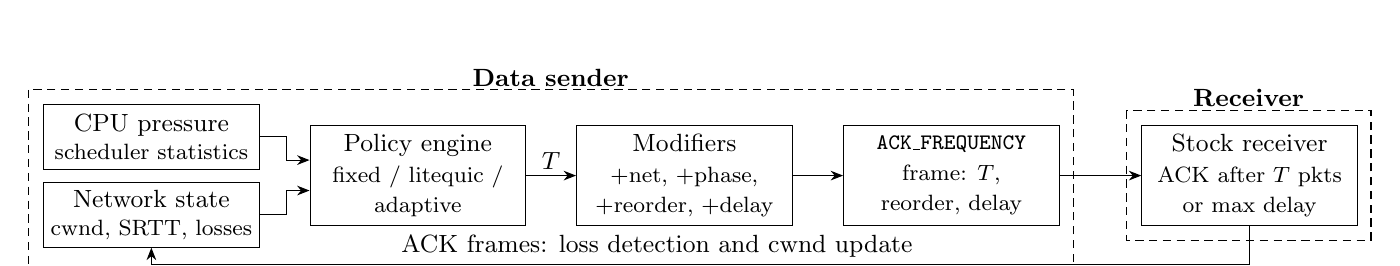
\begin{tikzpicture}[x=1pt, y=1pt, font=\small, >={Stealth[length=4.5pt,width=3.5pt]},
      box/.style={draw, align=center, inner sep=1pt, minimum width=77.9pt},
      main/.style={box, minimum height=36.2pt},
      input/.style={box, minimum height=23.3pt},
      group/.style={draw, dash pattern=on 3pt off 2pt}]
    % Data sender and receiver groups
    \draw[group] (0.9,-18.8) rectangle (378.5,-86.1);
    \node[anchor=south, font=\small\bfseries, inner sep=1pt] at (189.7,-18.8) {Data sender};
    \draw[group] (397.8,-26.2) rectangle (486.1,-73.1);
    \node[anchor=south, font=\small\bfseries, inner sep=1pt] at (441.9,-26.2) {Receiver};
    % Inputs
    \node[input] (cpu) at (45.4,-35.8) {CPU pressure\\[-1pt]\footnotesize scheduler statistics};
    \node[input] (net) at (45.4,-64.0) {Network state\\[-1pt]\footnotesize cwnd, SRTT, losses};
    % Decision chain
    \node[main] (pol) at (141.7,-49.8) {Policy engine\\\footnotesize fixed / litequic /\\\footnotesize adaptive};
    \node[main] (mod) at (238.0,-49.8) {Modifiers\\\footnotesize +net, +phase,\\\footnotesize +reorder, +delay};
    \node[main] (fr)  at (334.5,-49.8) {\footnotesize\texttt{ACK\_FREQUENCY}\\\footnotesize frame: $T$,\\\footnotesize reorder, delay};
    \node[main] (rx)  at (442.25,-49.8) {Stock receiver\\\footnotesize ACK after $T$ pkts\\\footnotesize or max delay};
    % Arrows
    \draw[->] (cpu.east) -- (94.2,-35.8) |- (pol.west |- 0,-44.2);
    \draw[->] (net.east) -- (94.2,-64.0) |- (pol.west |- 0,-55.2);
    \draw[->] (pol) -- node[above, inner sep=2pt] {$T$} (mod);
    \draw[->] (mod) -- (fr);
    \draw[->] (fr) -- (rx);
    \draw[->] (rx.south) -- (442.25,-82.0) -- (45.4,-82.0) -- (net.south);
    \node[inner sep=1pt] at (228.1,-75.3) {ACK frames: loss detection and cwnd update};
  \end{tikzpicture}}
  \caption{ACK-frequency control loop. Only the data sender is modified, and the receiver's ACKs
    update its network state.}
  \label{fig:loop}
\end{figure}

At process start, \pol{QuicMcnAckInitialize} reads the \pol{MCN\_ACK\_*} variables once. At
handshake confirmation, \pol{QuicConnMcnAckOnHandshakeConfirmed} sets the initial threshold. After
each receive-queue drain, \pol{QuicConnFlushRecv} calls \pol{QuicConnMcnAckOnRecvFlush}, which
runs the active policy. CPU inputs come from \path{/proc/thread-self/schedstat} and
\path{/proc/stat} (about 15\,$\mu$s per decision, at most once per 20\ms), network inputs from the
connection. \pol{QuicConnMcnAckSetThreshold} applies the
modifiers. Then \pol{QuicConnMcnAckUpdatePeer} schedules an \pol{ACK\_FREQUENCY} frame if a field
changed, which the unmodified receiver follows. We also time the receive path
(\pol{QuicConnFlushRecv}), ACK-frame handling (\pol{QuicLossDetection\allowbreak ProcessAckFrame}) and the
send path (\pol{QuicSendFlush}). In a download, the server receive time measures \emph{ACK
processing}, and the client send time measures \emph{ACK generation}. Both are elapsed times
without kernel UDP time and include preemption under load.

\subsection{Policy summary}
Table~\ref{tab:policies} summarises the policies and modifiers.

\begin{table}[H]
  \centering
  \small
  \caption{Policies and modifiers. Modifiers apply to the threshold chosen by any policy.}
  \label{tab:policies}
  \begin{tabularx}{\textwidth}{@{}p{2.65cm}p{5.5cm}X@{}}
    \toprule
    Policy & Decision basis & Main objective \\
    \midrule
    \pol{default}      & MsQuic's send-batching heuristic     & Unmodified MsQuic reference \\
    \pol{fixed:N}      & None (\pol{fixed:2} = RFC baseline)  & Isolate the effect of $T$ \\
    \pol{litequic}     & ACK frames per receive operation     & Infer CPU limitation from ACK backlog \\
    \pol{adaptive[:C]} & Thread and machine CPU pressure      & Reduce ACKs only when CPU is scarce \\
    \pol{+net}         & Congestion window, queuing, losses   & Keep at least four ACKs per window \\
    \pol{+phase}       & Cubic slow start and recovery        & Protect short transfers and loss recovery \\
    \pol{+reorder}     & RFC 9002 packet threshold (3)        & Skip immediate ACKs for harmless gaps \\
    \pol{+delay}       & Smoothed RTT                         & Bound the feedback gap below $T$ packets \\
    \bottomrule
  \end{tabularx}
\end{table}

\FloatBarrier
\section{Experimental Setup}\label{sec:setup}
\para{Wi-Fi testbed (Exps.~1--3).} The server has an AMD Ryzen 7 5800X (16 threads) running
Ubuntu 22.04 with 1\,Gb/s Ethernet. The client has an Intel i5-1335U on campus Wi-Fi. The Wi-Fi
link provides 460--660\mbps{} with a minimum RTT of 1.5--2.1\ms. Both run our MsQuic v2.6.3 build
from the same commit, with Cubic and pacing.

A CPU load of $K$x means $K$ busy-loop processes per logical CPU. The loops run in the same login
session as the server. Otherwise, Linux autogroup scheduling would isolate them from the QUIC
threads. At 4x load the QUIC thread wants a CPU 90\% of the time.

Experiment 1 downloads files of 20\,MB to 1\,GB with 12 policy variants (Table~\ref{tab:policies},
\pol{adaptive:255} and modifier combinations). It uses three load levels (none, 2x and 4x) and 3
repetitions; 420 of its 432 runs completed. Experiment 2 is a load sweep with 500\,MB files, 4
policies and seven loads from 0 to 4x, with 2 repetitions; 52 of 56 runs completed. Experiment 3
streams 40\,s of video in 2\,s segments at bitrates of 25--400\mbps{} with 8 policies; 64 of 72
sessions completed. The ABR algorithm
picks the highest bitrate that is at most $0.9\times$ the harmonic-mean throughput of the last 3
segments. The player uses a 10\,s buffer. QoE is computed per segment as the bitrate, minus the change
from the previous bitrate and a penalty of 400\mbps{} per second of startup delay and
rebuffering. Policies are interleaved and rotated between repetitions. Figures show a subset of the variants;
tables for all of them are in the repository.

\para{Lossy-path testbed (Exps.~4--6).} These experiments use a second server, an Intel i7-14700
(28 threads, Ubuntu 24.04) with a 100\,Mb/s Ethernet port, and the same Wi-Fi client. With
\pol{tbf} and \pol{netem} on the server's egress we emulate a 100\mbps{} bottleneck with 10\ms{} of
added delay (minimum RTT 11.5\ms), either without loss or with 0.1\% random loss. Every run
downloads a 100\,MB file. Experiment 4 sweeps \pol{fixed:2} to \pol{fixed:100} without CPU load.
Experiment 5 compares 8 policies on both paths at no load, 2x and 4x, with the load in the servers'
session as in Exps.~1--3. Experiment 6 sweeps the ceiling $C$ of \pol{adaptive} from 2 to 100 at
2x load on both paths, with no modifier and with \pol{+phase}, \pol{+delay}, \pol{+net} and all of
them. Exps.~4--5 use 3 repetitions and Exp.~6 uses 6 per path; none of the 618 runs stalled.

\para{Metrics.} Besides ACK counts and ACK-path times, we report goodput, completion time and the
10th percentile of 100\ms{} throughput (p10). A download \emph{collapses} when its p10 falls below 100\mbps. A run \emph{stalls} when
MsQuic's 16\,s disconnect timeout closes it because nothing was acknowledged; stalled runs are
excluded from all values and counted separately. Values are medians, with IQRs where $n \ge 3$.
Wi-Fi throughput varies by $\pm$5--15\% between runs, so we cannot resolve smaller differences.

\section{Results and Performance Analysis}\label{sec:results}
\subsection{File download performance}\label{sec:downloads}
ACK-path time measures the benefit of fewer ACKs; goodput and completion time measure the cost.

\begin{figure}[htbp]
  \centering
  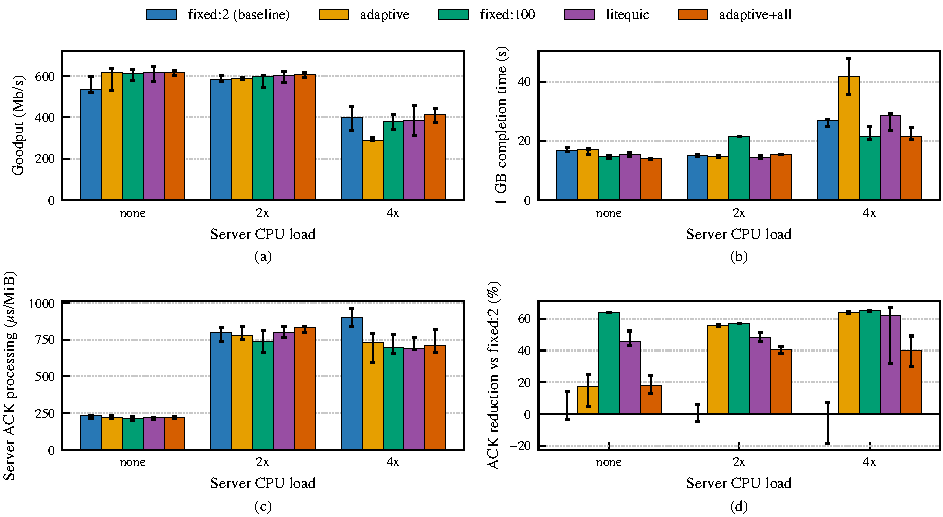
\includegraphics[width=\textwidth]{fig2_downloads}
  \caption{File downloads over Wi-Fi by server CPU load (Exp.~1, 500\,MB and 1\,GB files,
    $n{=}4$--6; (b) 1\,GB only, $n{=}1$--3). Bars: median; whiskers: IQR. (a) goodput; (b)
    completion time; (c) server ACK-processing time; (d) ACK frames removed relative to
    \pol{fixed:2} at the same load.}
  \label{fig:downloads}
\end{figure}

\para{Idle server.} On an idle server, \pol{adaptive} keeps $T{=}2$ (Figure~\ref{fig:downloads}d).
Its 13.0 ACKs/MiB versus 15.8 for \pol{fixed:2} is within noise. Even at $T{=}2$, MsQuic sends
only about one ACK per 50 data packets: it acknowledges once per receive batch, and Wi-Fi delivers
packets in bursts. This limits what any threshold can save on this path. \pol{litequic} reads the
same bursts as CPU limitation: it raises $T$ to a mean of 59 and changes it about 36 times per
second (61 under load). Idle goodput (536--619\mbps) varies within Wi-Fi noise.

\para{Threshold follows the load.} In the load sweep (Exp.~2), \pol{adaptive} keeps $T{=}2$ up to
0.25x load, uses 10 at 0.5x and 69 at 0.75x, and reaches its ceiling of about 100 from 1x, when the
machine is fully busy. Up to 2x, the goodput of all four policies stays within 10\% of
\pol{fixed:2}.

\para{Moderate contention.} At 2x load, \pol{adaptive} gives the best trade-off.
Figure~\ref{fig:downloads}(d) shows 56\% fewer ACKs than the baseline (5.8 vs.\ 13.2 per MiB).
Client ACK-generation time falls by 44\%, from 215 to 120\,$\mu$s/MiB.
Figure~\ref{fig:downloads}(c) shows only a 2\% drop in server ACK-processing time (796 to
781\,$\mu$s/MiB). At 50--100 packets per ACK, much of this work is per acknowledged packet.
Whole-process CPU did not change consistently, so these are ACK-path savings only.
Figures~\ref{fig:downloads}(a)--(b) show no cost: goodput is 588 vs.\ 582\mbps{} and the 1\,GB
completion time 14.7 vs.\ 15.1\,s. A ceiling of 255 removes 78\% of ACKs but lowers goodput to
545\mbps{} and p10 throughput to 386\mbps{} (baseline 511).

\para{Severe contention.} At 4x load the baseline drops to 401\mbps. \pol{adaptive} runs at a
threshold of about 100 and removes 64\% of ACKs (Figure~\ref{fig:downloads}d).
Figure~\ref{fig:downloads}(c) shows a 19\% cut in server ACK-processing time (730 vs.\
900\,$\mu$s/MiB). However, Figures~\ref{fig:downloads}(a)--(b) show its goodput falling to
290\mbps{} and its 1\,GB download taking 41.8\,s instead of 26.8\,s.

Throughput dips of 1--15\,s cause this loss. A CPU-starved sender sends fewer than $T$ packets
per RTT, so the receiver waits for its 25\ms{} timer while the ACK-clocked sender idles. Among the 12
large downloads per policy on the loaded server, a download collapsed once with \pol{adaptive} and
\pol{fixed:100} and three times with \pol{adaptive:255}, but never with \pol{fixed:2},
\pol{litequic} or any variant with \pol{+delay}.

\pol{adaptive+all} keeps feedback timely. Its window-based ceiling keeps $T$ near 80, and its
SRTT/4 timer requests an ACK within 1--3\ms. It reaches 412\mbps{} and completes the 1\,GB download
in 21.6\,s with 40\% fewer ACKs. Without \pol{+net} ($T{\approx}93$),
\pol{adaptive+phase+reorder+delay} reaches 396\mbps{} with 39\% fewer ACKs, suggesting that the
short ACK timer matters most. The load sweep did not reproduce \pol{adaptive}'s median penalty (421 vs.\
366\mbps, $n{\le}2$), so the dips are the consistent signal.

\para{Stalls.} 24 of the 560 runs (4.3\%) stalled, all but one under CPU load. They hit 10 of the
12 variants, including \pol{fixed:2}, so we do not attribute them to the threshold.

\FloatBarrier
\subsection{Video streaming performance}
Each video segment is a 6--100\,MB transfer after an idle gap that spends much of its time in slow
start, so it is more sensitive to $T$ than a long download. No completed session rebuffered.

\begin{figure}[htbp]
  \centering
  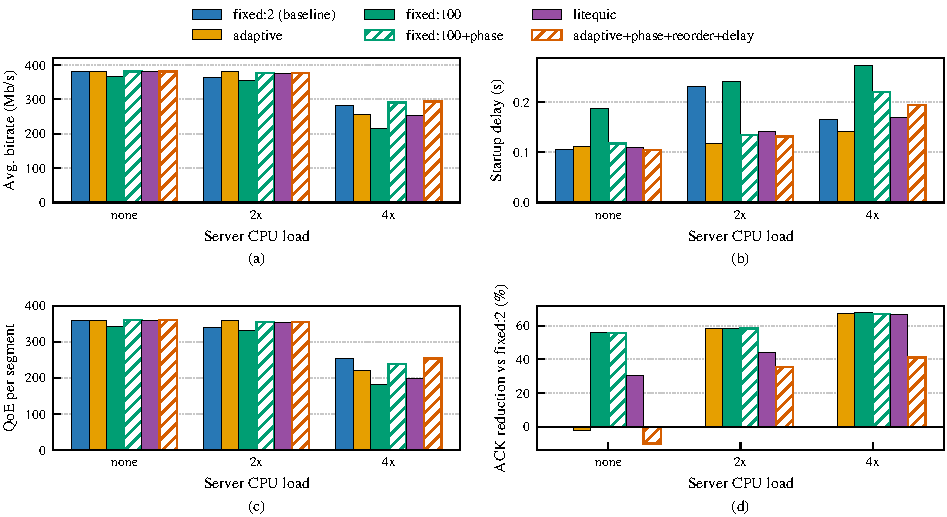
\includegraphics[width=\textwidth]{fig3_video}
  \caption{Video streaming over Wi-Fi (Exp.~3, medians of $n{=}1$--3 completed sessions per bar; 64
    of 72 sessions completed). (a) average delivered bitrate (maximum achievable 381\mbps); (b)
    startup delay; (c) linear QoE per segment; (d) ACK reduction vs.\ \pol{fixed:2}. Hatched bars:
    \pol{+phase} variants.}
  \label{fig:video}
\end{figure}

\pol{fixed:100} performs worst at every load. Figure~\ref{fig:video}(b) shows its startup delays of
0.19, 0.24 and 0.27\,s at no load, 2x and 4x. Figure~\ref{fig:video}(c) shows its QoE of 344, 333
and 182, against 360, 340 and 253 for \pol{fixed:2}. Here $T$ exceeds the slow-start window, so
the receiver waits for its timer. Phase awareness fixes this. \pol{fixed:100+phase} keeps the same
56--67\% ACK reduction (Figure~\ref{fig:video}d) but restores startup to 0.12 and 0.13\,s and QoE
to 360 and 355 at no load and 2x.

At 2x load, \pol{adaptive} performs best. Figure~\ref{fig:video}(a) shows the top bitrate of
381\mbps, with a 0.12\,s startup delay. Its QoE is 360 (baseline 340) with 58\% fewer ACKs.

At 4x load, \pol{adaptive+phase+reorder+delay} matches the baseline's QoE (254 vs.\ 253) and
bitrate (294 vs.\ 281\mbps) with 41\% fewer ACKs, but on two sessions only: three of its six
sessions under load stalled. Plain \pol{adaptive} and \pol{litequic} remove
67--68\% of ACKs, but their QoE drops to 220 and 199. Under CPU starvation, \pol{+phase} and
\pol{+delay} keep each segment's ramp-up and feedback timely.

\FloatBarrier
\subsection{Performance on a lossy path}\label{sec:loss}
Exps.~4--6 test whether a large threshold is safe when the path loses packets: first with fixed
thresholds on an idle server, then with the policies under CPU load, where \pol{adaptive} raises
$T$ because the CPU is busy, not because the path allows it.

\begin{figure}[htbp]
  \centering
  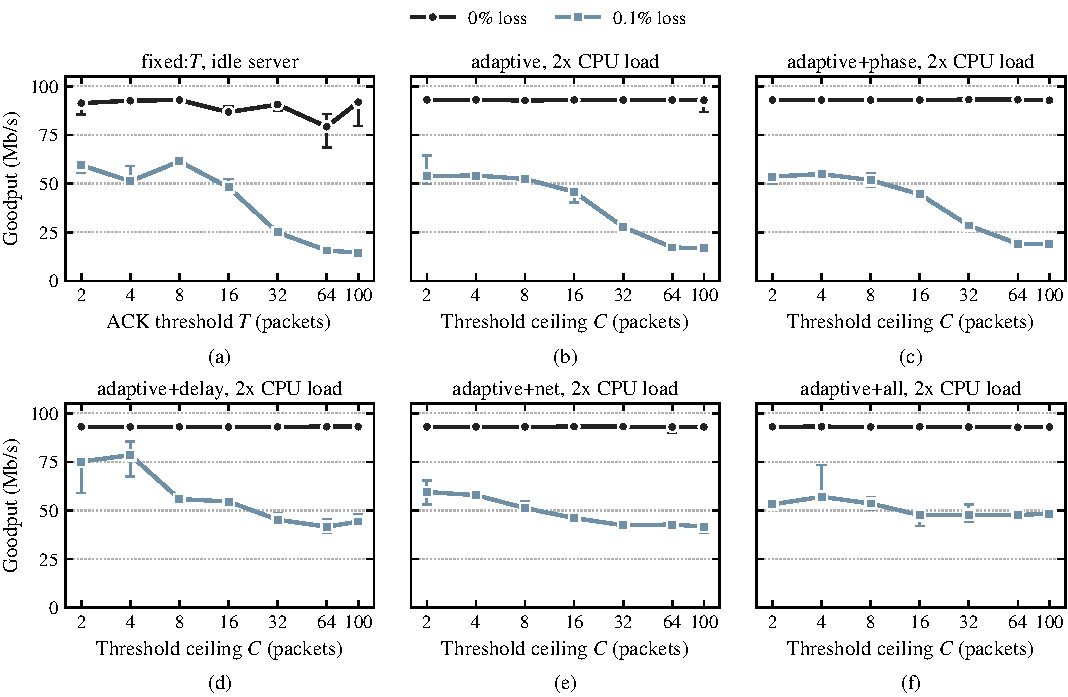
\includegraphics[width=0.96\textwidth]{fig4_threshold_loss}
  \caption{Goodput vs.\ ACK threshold on the emulated 100\mbps, +10\ms{} path with 0\% and 0.1\%
    random loss (100\,MB downloads; medians, whiskers: IQR). (a) \pol{fixed:}$T$, idle server
    (Exp.~4, $n{=}3$). (b)--(f) \pol{adaptive} with each modifier set at 2x CPU load vs.\ its
    ceiling $C$, which $T$ reaches unless \pol{+net} caps it (Exp.~6, $n{=}6$).}
  \label{fig:threshold}
\end{figure}

\para{Fixed thresholds.} Without loss, every threshold from 2 to 100 reaches 79--93\mbps{}
(Figure~\ref{fig:threshold}a). On this path $T{=}2$ yields one ACK per 4--5 packets, not one per
50 as on Wi-Fi (\S\ref{sec:downloads}), so a large $T$ saves far more ACK work: $T{=}100$ removes
95\% of ACKs and cuts server ACK-processing time by 59\% and client ACK-generation time by 91\%.
With 0.1\% loss, $T{\le}8$ stays within the run-to-run variation of $T{=}2$ (51--61 vs.\
59\mbps), and $T{=}8$ already removes 57\% of ACKs. Beyond that, goodput falls to 48\mbps{} at
$T{=}16$ and to 14.5\mbps{} at $T{=}100$, a 76\% loss. Sparse ACKs delay loss detection and slow down every recovery.

\para{Idle server and clean path.} In Exp.~5, without CPU load, \pol{adaptive}, all its variants
and \pol{litequic} keep $T{\approx}2$ and match \pol{fixed:2} on both paths. Under load on the clean
path, every variant reaches 93\mbps{} at every ceiling, like \pol{fixed:2}
(Figure~\ref{fig:threshold}b--f, 0\% loss), while its ACK reduction grows with $C$ to 82--94\% at
$C{=}100$. There, \pol{adaptive} cuts server ACK-processing time by 65\% and client ACK-generation
time by 91\%; \pol{adaptive+all}, whose window bound keeps $T$ near 34, cuts them by 55\% and
77\%. Where ACKs are frequent, reducing them saves substantial CPU at no cost in goodput.

\para{Lossy path under load.} Here CPU pressure alone fails. Under load, \pol{adaptive} raises
$T$ to its ceiling, so its goodput follows the fixed-threshold curve
(Figure~\ref{fig:threshold}b vs.\ a). Up to $C{=}8$ it matches \pol{fixed:2} (52--54 vs.\
50.5\mbps) with up to 59\% fewer ACKs, but at $C{\ge}64$ it falls to 17\mbps, a 67\% loss.
\pol{+phase} does not change this (Figure~\ref{fig:threshold}c, 19\mbps), because $T{=}2$ applies
only during each recovery period. The other modifiers make large ceilings safe. \pol{+net}
(Figure~\ref{fig:threshold}e) caps $T$ near 15 after congestion events, so from $C{=}16$ on its
goodput stays at 42--46\mbps{} with 76--78\% fewer ACKs. \pol{+delay} (Figure~\ref{fig:threshold}d)
requests an ACK within SRTT/4, about 3\ms, which limits the gap between ACKs to about 12 packets;
from $C{=}16$ on it keeps 42--55\mbps{} with 72--74\% fewer ACKs. Combining both,
\pol{adaptive+all} (Figure~\ref{fig:threshold}f) comes closest to the baseline: 48--49\mbps{}
(94--96\%) at every $C{\ge}16$, with 67--69\% fewer ACKs, 45--49\% less server ACK-processing time
and 59--62\% less client ACK-generation time. The modifiers thus trade part of the ACK reduction
(69--78\% instead of 93\%) for nearly all of the goodput, and they cost nothing on the clean path.
The remaining gap comes from where the bounds settle: thresholds up to 8 cost nothing at 0.1\%
loss (Figure~\ref{fig:threshold}a--b), but the bounds settle near $T{=}16$, at the knee of the
curve; a ceiling that shrinks with the measured loss rate could close it.

Exp.~5 confirms this with $C{=}100$ at 2x and 4x load: \pol{adaptive} falls to 16\mbps,
\pol{adaptive+all} keeps 79--84\% of \pol{fixed:2}'s goodput with 65--66\% fewer ACKs, and
\pol{litequic} ($T{\approx}3$) removes only 5--15\% of ACKs. One anomaly: with \pol{+delay} alone and $C{\le}4$, 8 of 12 lossy runs filled the bottleneck
queue (SRTT 24--41 vs.\ 13\ms), lost 4--6 times more packets and reached 73--90\mbps{}
(Figure~\ref{fig:threshold}d), a mode seen in only 13 of the other 204 lossy runs and never with
\pol{fixed:2}; we could not explain it and do not count it as a gain.

\FloatBarrier
\subsection{Overall policy comparison}
\begin{figure}[htbp]
  \centering
  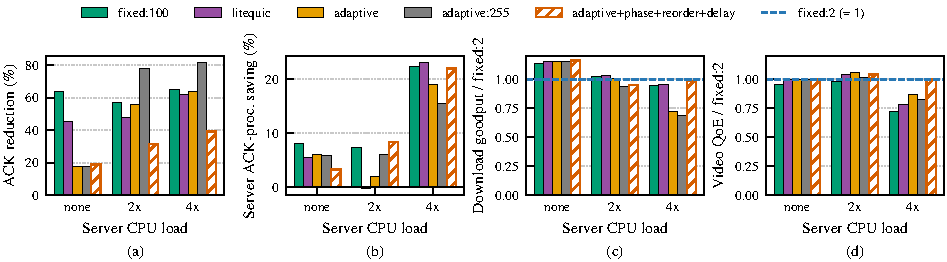
\includegraphics[width=\textwidth]{fig5_overall}
  \caption{Overall comparison relative to \pol{fixed:2} at the same CPU load (ratios of medians).
    (a)--(c) downloads of 500\,MB and 1\,GB (Exp.~1); (d) video sessions (Exp.~3). Dashed line:
    \pol{fixed:2}.}
  \label{fig:overall}
\end{figure}

Figure~\ref{fig:overall} summarises the trade-offs. At no load, goodput ratios above 1 reflect
Wi-Fi variation in the baseline runs, not a policy effect. At 2x load, \pol{adaptive} gives the
best balance. It removes over half of the ACKs while keeping goodput and QoE at or above the
baseline. At 4x load, the policies that hold large thresholds remove the most ACKs but lose goodput
and QoE. \pol{adaptive+phase+reorder+delay} removes fewer ACKs but is the only variant in
Figure~\ref{fig:overall} that keeps both at the baseline level. Server ACK-processing savings stay small except at 4x load
(Figure~\ref{fig:overall}b). No policy dominates, because the threshold that saves the most CPU
also delays feedback when the sender is starved or the path is lossy.

\FloatBarrier
\section{Limitations and Future Work}
\enlargethispage{\baselineskip} % keeps the last reference on page 9
Our results come from small samples ($n{=}2$--6 per Wi-Fi cell, $n{=}3$--6 in Exps.~4--6) with
single connections and Cubic, and one client. CPU contention came from busy loops, and
4.3\% of the Wi-Fi runs stalled for reasons we could not explain (\S\ref{sec:downloads}). The ceiling of 100 and other constants were
chosen by hand. We emulated only one lossy path (100\mbps, +10\ms, 0.1\% random loss). As
future work, we plan a full matrix of bandwidth, RTT, loss and CPU load to find the best threshold
for each condition. These data could then train a lightweight MLP that predicts $T$ from CPU
pressure, bandwidth, SRTT, loss and the congestion window. Its output would be clipped to
$[2, \mathrm{cwnd}_{\mathrm{pkts}}/4]$ and reset to 2 after a loss. Both extensions are proposed
and not yet implemented.

\section{Conclusion and Individual Contributions}
We showed that a QUIC sender can choose its ACK frequency at run time with only standard
\pol{ACK\_FREQUENCY} frames and an unmodified receiver. Our CPU-aware \pol{adaptive} policy keeps
full RFC feedback on an idle server and reduces ACK work only when the CPU is scarce. Under moderate
load it lowers ACK overhead without hurting download or video performance. Under severe load, a
large threshold alone causes throughput collapses. Bounding the threshold by the congestion window
and scaling the ACK delay with the RTT keep feedback timely and preserve performance. A ceiling of
255 removed the most ACKs but caused the most collapses, so the ceiling should stay near 100 or
follow the congestion window. On a
lossy path, a CPU-driven threshold alone loses two thirds of the goodput, while bounding it by the
congestion window and the RTT keeps 79--96\% of it with two thirds fewer ACKs. Network conditions
must therefore constrain any CPU-driven choice of the ACK threshold.

\para{Individual contributions.} \emph{Kunal Umaji} built the base MsQuic implementation. Kunal
added the policy framework, the \pol{ACK\_FREQUENCY} update path and the ACK-cost instrumentation,
and modified MsQuic so that policies can be selected at run time. \emph{Aravindh Sriram Kumar A G}
designed and implemented the CPU-aware \pol{adaptive} policy and its network-aware \pol{+net}
ceiling. Aravindh evaluated these policies and analysed why they succeed under moderate load and
need feedback constraints under severe load and loss. \emph{Kaveenraj G} implemented the
LiteQUIC-inspired policy and the \pol{+phase}, \pol{+reorder} and \pol{+delay} modifiers. Kaveenraj
evaluated these policies and analysed their effect on short transfers, video QoE and feedback
timeliness.

\para{Repository and reproduction.} The code is at \url{https://github.com/kunalumaji/mcn26}
(branch \pol{staging}). Build MsQuic and the \pol{quicfile} tool on both machines with
\path{scripts/setup.sh}. Run all experiments with \path{experiments/run_all.sh}; Exps.~4--6 emulate the path with
\path{scripts/netem.sh}.

% References in the proposal's style, numbered in order of first citation.
{\small
\begin{thebibliography}{9}
\setlength{\itemsep}{1pt}\setlength{\parsep}{0pt}
\bibitem{zhang2024quic} X. Zhang, S. Jin, Y. He, A. Hassan, Z. M. Mao, F. Qian, and Z.-L. Zhang.
  ``QUIC is not Quick Enough over Fast Internet,'' \emph{Proceedings of the ACM Web Conference
  (WWW)}, 2024.
\bibitem{bi2024litequic} P. Bi, Y. Zou, M. Xiao, D. Yu, Y. Li, Z. Liu, and Q. Xie. ``LiteQUIC:
  Improving QoE of Video Streams by Reducing CPU Overhead of QUIC,'' \emph{Proceedings of the 32nd
  ACM International Conference on Multimedia (MM)}, 2024.
\bibitem{rfc9000} J. Iyengar and M. Thomson. ``QUIC: A UDP-Based Multiplexed and Secure
  Transport,'' \emph{RFC 9000}, IETF, 2021.
\bibitem{rfc9002} J. Iyengar and I. Swett. ``QUIC Loss Detection and Congestion Control,''
  \emph{RFC 9002}, IETF, 2021.
\bibitem{ackfreq14} J. Iyengar, I. Swett, and M. K\"uhlewind. ``QUIC Acknowledgment Frequency,''
  \emph{Internet-Draft draft-ietf-quic-ack-frequency-14}, IETF, 2026.
\bibitem{custura2023ackfreq} A. Custura, T. Jones, R. Secchi, and G. Fairhurst. ``Reducing the
  Acknowledgement Frequency in IETF QUIC,'' \emph{International Journal of Satellite Communications
  and Networking}, vol.~41, no.~4, pp.~315--330, 2023.
\end{thebibliography}
}

\end{document}
